\begin{figure}
	\centering
	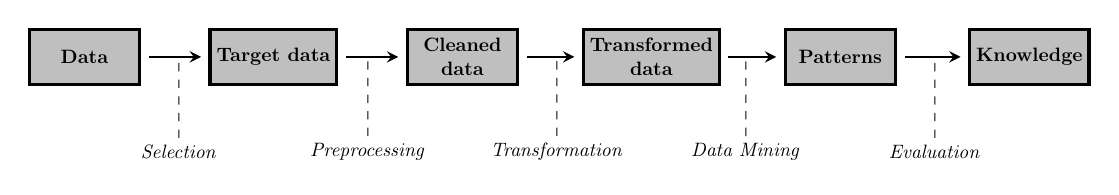
\begin{tikzpicture}[
		scale=0.4,
		every node/.append style={scale=0.7},
		box/.style={draw=black,very thick,minimum width=2cm,minimum height=1cm,align=center,fill=lightgray},
		arr/.style={thick,-stealth,shorten >= 1mm,shorten <= 1mm}
	]
		
		\node[box] (A) at (0,0) {\textbf{Data}};
		\node[box] (B) at (6,0) {\textbf{Target data}};
		\node[box] (C) at (12,0) {\textbf{Cleaned} \\ \textbf{data}};
		\node[box] (D) at (18,0) {\textbf{Transformed} \\ \textbf{data}};
		\node[box] (E) at (24,0) {\textbf{Patterns}};
		\node[box] (F) at (30,0) {\textbf{Knowledge}};

		\draw[arr] (A) -- (B);
		\draw[arr] (B) -- (C);
		\draw[arr] (C) -- (D);
		\draw[arr] (D) -- (E);
		\draw[arr] (E) -- (F);

		\node (a) at (3,-3) {\textit{Selection}};
		\node (b) at (9,-3) {\textit{Preprocessing}};
		\node (c) at (15,-3) {\textit{Transformation}};
		\node (d) at (21,-3) {\textit{Data Mining}};
		\node (e) at (27,-3) {\textit{Evaluation}};

		\draw[dashed] (a) -- ++(0,3);
		\draw[dashed] (b) -- ++(0,3);
		\draw[dashed] (c) -- ++(0,3);
		\draw[dashed] (d) -- ++(0,3);
		\draw[dashed] (e) -- ++(0,3);
		
	\end{tikzpicture}
\end{figure}